% Title:
% 	CheatSheet
% -------------------------------------------------
% Description:
% 	Template for cheat sheets.
%
% Creator: Tommy O.

% -------------------------------------------------
% Package imports
% -------------------------------------------------
\documentclass[11pt, a4paper]{article}
\usepackage[utf8]{inputenc}% Input encoding
\usepackage[english]{babel}% Set language to english
\usepackage{graphicx}% For importing graphics
\usepackage{amsthm, amsfonts, amssymb}% All the AMS packages
\usepackage{mathtools}% Fixes a few AMS bugs
\usepackage[expansion=false]{microtype}% Fixes to make typography better
\usepackage{hyperref}% For \href{URL}{text}
\usepackage{fancyhdr}% For fancy headers
\usepackage[sharp]{easylist}% Easy nested lists
\usepackage{parskip}% Web-like paragraphs
\usepackage{multicol}% For multiple columns
\usepackage{tikz-cd}% For diagrams
\usepackage{listings}% To include source-code
\usepackage[margin = 1.2cm]{geometry}% May be used to set margins
\usepackage{nicefrac}% Enables \nicefrac{nom}{denom}
%\usepackage[sc]{mathpazo}% A nice font, alternative to CM

% -------------------------------------------------
% Package setup
% -------------------------------------------------
\newcommand{\Title}{Cheat Sheet SUBJECT}
\newcommand{\Subtitle}{SUBTITLE}
\newcommand{\Author}{Tommy O}
\newcommand{\listSpace}{-0.2em}% Global list space

% Shortcuts for sets in mathematics
\newcommand{\Q}{\mathbb{Q}}
\newcommand{\R}{\mathbb{R}}
\newcommand{\C}{\mathbb{C}}
\newcommand{\Z}{\mathbb{Z}}

% Change the section command to inluce lines, save space, etc.
\usepackage{titlesec}
\titlespacing\paragraph{0pt}{6pt plus 4pt minus 2pt}{8pt plus 4pt minus 2pt}
\titleformat{\section}
{\normalfont\Large\bfseries}{\thesection}{0em}{$\vartriangleright$ }[{\titlerule[1.2pt]}]

% -------------------------------------------------
% Document start
% -------------------------------------------------
\begin{document}
	\pagestyle{empty}
\noindent
\begin{minipage}[t]{.75\textwidth}
	\raggedright
	{\huge \scshape \Title} \\
	{\small \itshape \Subtitle \hspace{1ex}-- \Author \hspace{1ex}-- {\footnotesize Last edit: \today}}
\end{minipage}%
\begin{minipage}[t]{.25\textwidth}
	\raggedleft
	
\includegraphics[width=2.5cm]{figs/logo.pdf}
\end{minipage} 
\vspace{0.1em} 
\hrule\hrule

% -------------------------------------------------
% Document content start
% -------------------------------------------------
\section*{An introductory section}
Plug the series expansion into the equation, collect powers of $\epsilon$ and 
set to 0.
Let $A(T)$ and $B(T)$ be constants of the slow time.
Set coefficients of forcing terms to zero to avoid resonance.
Find $A(0)$ and $A(0)$ using $0 = x(0, \epsilon) = x_0 (0, 0) + \epsilon x_1 (0, 0) + \dots$. This implies that all $x_i(0,0) = 0$.
\begin{multicols}{2}
\section*{Phase plane ($\mathbb{R}^2$)}
\begin{easylist}[itemize]
	\ListProperties(Space=\listSpace, Space*=\listSpace)
	# A good website for plotting phase planes is \url{http://comp.uark.edu/~aeb019/pplane.html}.
	# Quantitative behavior with exact formulas is often unattainable,
	so we settle for qualitative behavior.
	# \textbf{Nulliclines} are curves where either $\dot{x} = 0$ or $\dot{y} = 
	0$.
\end{easylist}

\section*{Limit cycles(closed orbits)}
\begin{easylist}[itemize]
	\ListProperties(Space=\listSpace, Space*=\listSpace)
	# \textbf{Ruling out closed orbits}:
	## If $\dot{\mathbf{x}} = - \nabla V$ (\textbf{gradient system}) there are no closed orbits.
	## If there exists a \textbf{Liapunov function} there is no closed orbit.
	A Liapunov function has:
	\begin{easylist}[enumerate]
		\ListProperties(Space=\listSpace, Space*=\listSpace)
		### $V(\mathbf{x}) > 0$ for all $\mathbf{x} \neq \mathbf{x}^*$(pos.def).
		### $\dot{V}(\mathbf{x}) < 0$ for all $\mathbf{x}$ (downhill flow)
	\end{easylist}
\end{easylist}
\begin{easylist}[itemize]
	\ListProperties(Space=\listSpace, Space*=\listSpace)
	## \textbf{Dulac's criterion} states that if $\nabla \cdot \left(g \dot{\mathbf{x}}\right)$
	has one sign there are no closed orbits. This is from the div. theorem:
	\begin{equation*}
		\iint \nabla \cdot \mathbf{F} \ dA = \oint \mathbf{F} \cdot\hat{\mathbf{n}} \ dr
	\end{equation*}
	
	# \textbf{Finding closed orbits}:
	## The \textbf{Poincaré-Bendixson theorem} states that if one can construct a trapping
	region then $\Omega$ must have a limit cycle.
	\begin{center}
		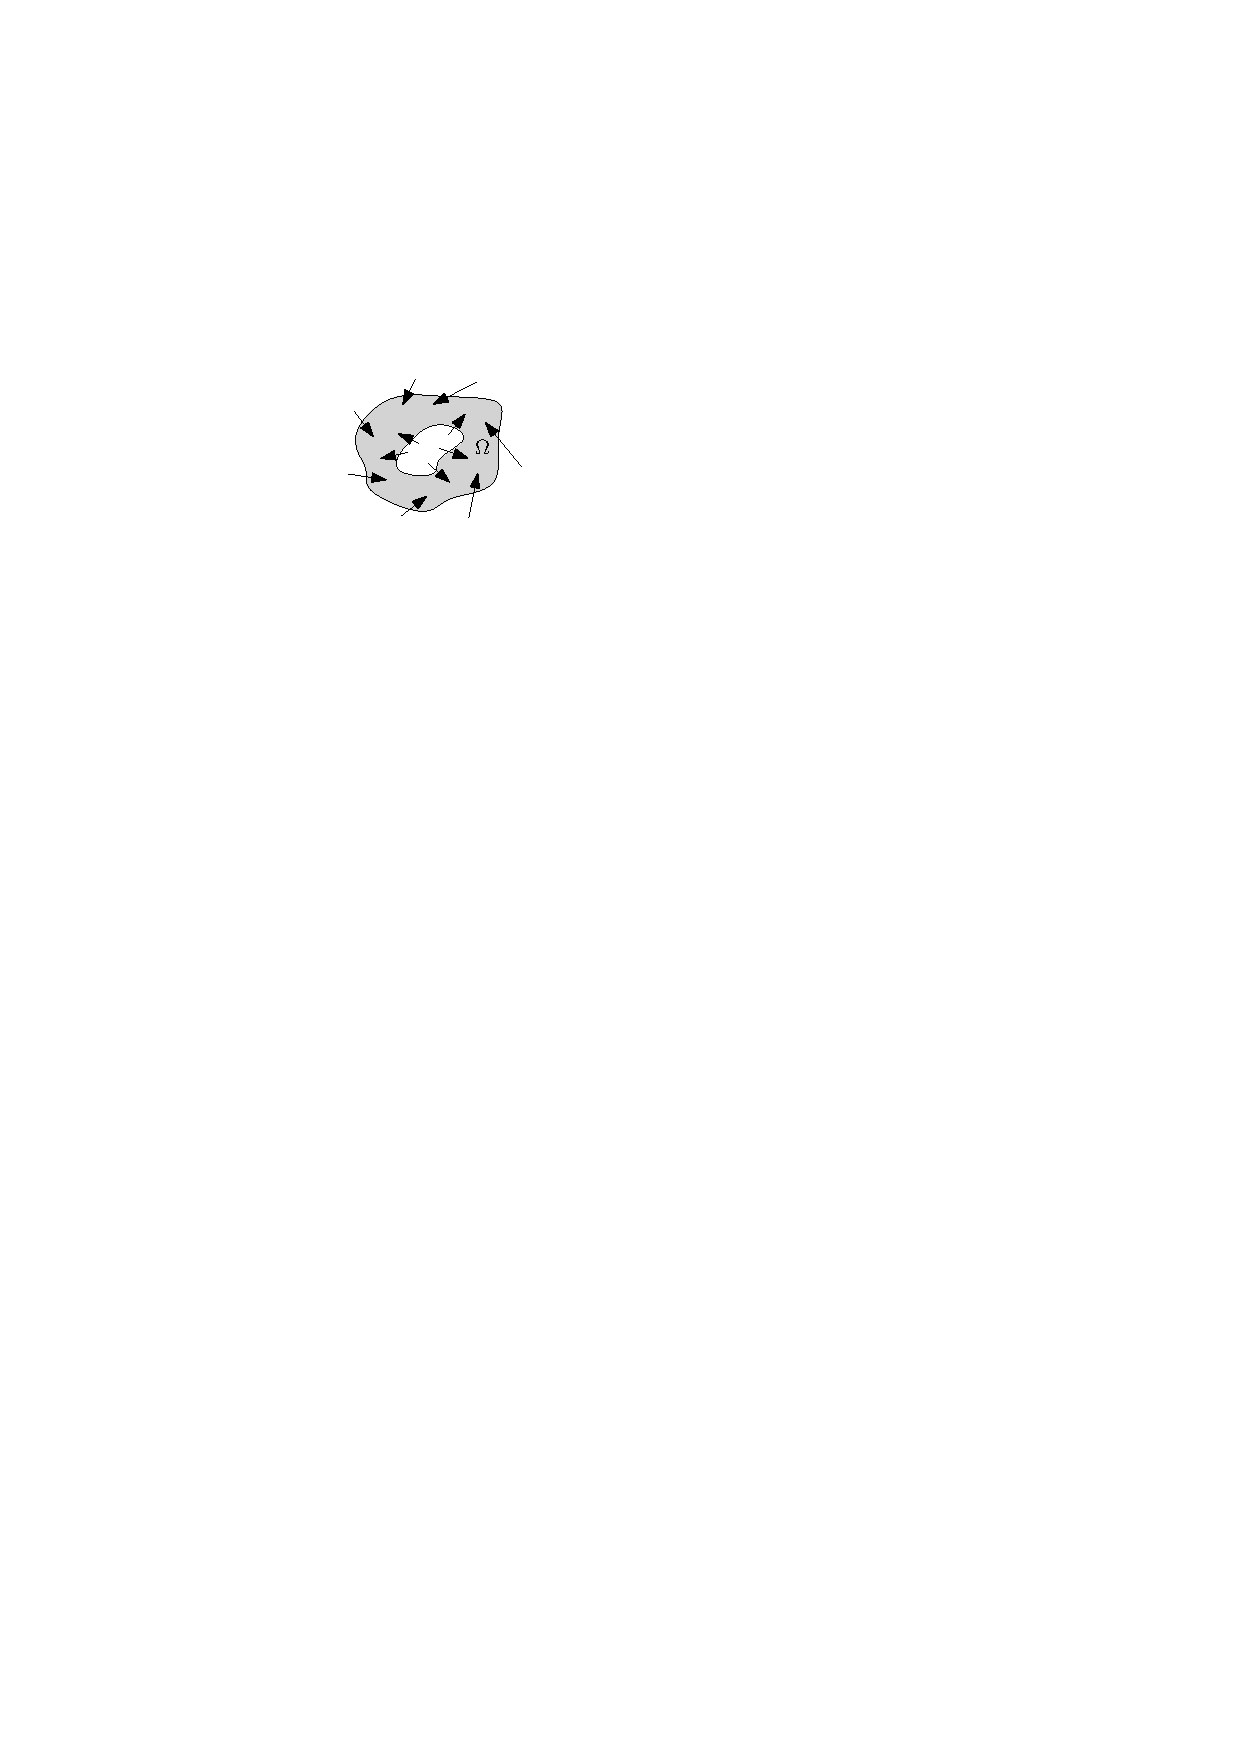
\includegraphics[width=3.5cm]{figs/trapping}
	\end{center}

	# \textbf{Relaxation oscillations} operate on two time scales; a slow 
	buildup and a fast release.
\end{easylist}

\section*{References}
\small
\begin{easylist}[itemize]
	\ListProperties(Space=\listSpace, Space*=\listSpace)
	# Book number one.
	# Book number two.
\end{easylist}
\end{multicols}

\end{document}